
%% bare_conf.tex
%% V1.3
%% 2007/01/11
%% by Michael Shell
%% See:
%% http://www.michaelshell.org/
%% for current contact information.
%%
%% This is a skeleton file demonstrating the use of IEEEtran.cls
%% (requires IEEEtran.cls version 1.7 or later) with an IEEE conference paper.
%%
%% Support sites:
%% http://www.michaelshell.org/tex/ieeetran/
%% http://www.ctan.org/tex-archive/macros/latex/contrib/IEEEtran/
%% and
%% http://www.ieee.org/

%%*************************************************************************
%% Legal Notice:
%% This code is offered as-is without any warranty either expressed or
%% implied; without even the implied warranty of MERCHANTABILITY or
%% FITNESS FOR A PARTICULAR PURPOSE! 
%% User assumes all risk.
%% In no event shall IEEE or any contributor to this code be liable for
%% any damages or losses, including, but not limited to, incidental,
%% consequential, or any other damages, resulting from the use or misuse
%% of any information contained here.
%%
%% All comments are the opinions of their respective authors and are not
%% necessarily endorsed by the IEEE.
%%
%% This work is distributed under the LaTeX Project Public License (LPPL)
%% ( http://www.latex-project.org/ ) version 1.3, and may be freely used,
%% distributed and modified. A copy of the LPPL, version 1.3, is included
%% in the base LaTeX documentation of all distributions of LaTeX released
%% 2003/12/01 or later.
%% Retain all contribution notices and credits.
%% ** Modified files should be clearly indicated as such, including  **
%% ** renaming them and changing author support contact information. **
%%
%% File list of work: IEEEtran.cls, IEEEtran_HOWTO.pdf, bare_adv.tex,
%%                    bare_conf.tex, bare_jrnl.tex, bare_jrnl_compsoc.tex
%%*************************************************************************

% *** Authors should verify (and, if needed, correct) their LaTeX system  ***
% *** with the testflow diagnostic prior to trusting their LaTeX platform ***
% *** with production work. IEEE's font choices can trigger bugs that do  ***
% *** not appear when using other class files.                            ***
% The testflow support page is at:
% http://www.michaelshell.org/tex/testflow/



% Note that the a4paper option is mainly intended so that authors in
% countries using A4 can easily print to A4 and see how their papers will
% look in print - the typesetting of the document will not typically be
% affected with changes in paper size (but the bottom and side margins will).
% Use the testflow package mentioned above to verify correct handling of
% both paper sizes by the user's LaTeX system.
%
% Also note that the "draftcls" or "draftclsnofoot", not "draft", option
% should be used if it is desired that the figures are to be displayed in
% draft mode.
%
\documentclass[10pt, conference, compsocconf]{IEEEtran}
% Add the compsocconf option for Computer Society conferences.
%
% If IEEEtran.cls has not been installed into the LaTeX system files,
% manually specify the path to it like:
% \documentclass[conference]{../sty/IEEEtran}





% Some very useful LaTeX packages include:
% (uncomment the ones you want to load)


% *** MISC UTILITY PACKAGES ***
%
%\usepackage{ifpdf}
% Heiko Oberdiek's ifpdf.sty is very useful if you need conditional
% compilation based on whether the output is pdf or dvi.
% usage:
% \ifpdf
%   % pdf code
% \else
%   % dvi code
% \fi
% The latest version of ifpdf.sty can be obtained from:
% http://www.ctan.org/tex-archive/macros/latex/contrib/oberdiek/
% Also, note that IEEEtran.cls V1.7 and later provides a builtin
% \ifCLASSINFOpdf conditional that works the same way.
% When switching from latex to pdflatex and vice-versa, the compiler may
% have to be run twice to clear warning/error messages.






% *** CITATION PACKAGES ***
%
%\usepackage{cite}
% cite.sty was written by Donald Arseneau
% V1.6 and later of IEEEtran pre-defines the format of the cite.sty package
% \cite{} output to follow that of IEEE. Loading the cite package will
% result in citation numbers being automatically sorted and properly
% "compressed/ranged". e.g., [1], [9], [2], [7], [5], [6] without using
% cite.sty will become [1], [2], [5]--[7], [9] using cite.sty. cite.sty's
% \cite will automatically add leading space, if needed. Use cite.sty's
% noadjust option (cite.sty V3.8 and later) if you want to turn this off.
% cite.sty is already installed on most LaTeX systems. Be sure and use
% version 4.0 (2003-05-27) and later if using hyperref.sty. cite.sty does
% not currently provide for hyperlinked citations.
% The latest version can be obtained at:
% http://www.ctan.org/tex-archive/macros/latex/contrib/cite/
% The documentation is contained in the cite.sty file itself.



% Graphics
\usepackage[pdftex]{graphicx}
%\usepackage[tight,footnotesize]{subfigure}
\usepackage{subfigure}

%Table background
\usepackage[table,xcdraw]{xcolor}
% *** GRAPHICS RELATED PACKAGES ***

%degree com
\usepackage{gensymb}




% *** GRAPHICS RELATED PACKAGES ***
%
\ifCLASSINFOpdf
  % \usepackage[pdftex]{graphicx}
  % declare the path(s) where your graphic files are
  % \graphicspath{{../pdf/}{../jpeg/}}
  % and their extensions so you won't have to specify these with
  % every instance of \includegraphics
  % \DeclareGraphicsExtensions{.pdf,.jpeg,.png}
\else
  % or other class option (dvipsone, dvipdf, if not using dvips). graphicx
  % will default to the driver specified in the system graphics.cfg if no
  % driver is specified.
  % \usepackage[dvips]{graphicx}
  % declare the path(s) where your graphic files are
  % \graphicspath{{../eps/}}
  % and their extensions so you won't have to specify these with
  % every instance of \includegraphics
  % \DeclareGraphicsExtensions{.eps}
\fi
% graphicx was written by David Carlisle and Sebastian Rahtz. It is
% required if you want graphics, photos, etc. graphicx.sty is already
% installed on most LaTeX systems. The latest version and documentation can
% be obtained at: 
% http://www.ctan.org/tex-archive/macros/latex/required/graphics/
% Another good source of documentation is "Using Imported Graphics in
% LaTeX2e" by Keith Reckdahl which can be found as epslatex.ps or
% epslatex.pdf at: http://www.ctan.org/tex-archive/info/
%
% latex, and pdflatex in dvi mode, support graphics in encapsulated
% postscript (.eps) format. pdflatex in pdf mode supports graphics
% in .pdf, .jpeg, .png and .mps (metapost) formats. Users should ensure
% that all non-photo figures use a vector format (.eps, .pdf, .mps) and
% not a bitmapped formats (.jpeg, .png). IEEE frowns on bitmapped formats
% which can result in "jaggedy"/blurry rendering of lines and letters as
% well as large increases in file sizes.
%
% You can find documentation about the pdfTeX application at:
% http://www.tug.org/applications/pdftex





% *** MATH PACKAGES ***
%
%\usepackage[cmex10]{amsmath}
% A popular package from the American Mathematical Society that provides
% many useful and powerful commands for dealing with mathematics. If using
% it, be sure to load this package with the cmex10 option to ensure that
% only type 1 fonts will utilized at all point sizes. Without this option,
% it is possible that some math symbols, particularly those within
% footnotes, will be rendered in bitmap form which will result in a
% document that can not be IEEE Xplore compliant!
%
% Also, note that the amsmath package sets \interdisplaylinepenalty to 10000
% thus preventing page breaks from occurring within multiline equations. Use:
%\interdisplaylinepenalty=2500
% after loading amsmath to restore such page breaks as IEEEtran.cls normally
% does. amsmath.sty is already installed on most LaTeX systems. The latest
% version and documentation can be obtained at:
% http://www.ctan.org/tex-archive/macros/latex/required/amslatex/math/





% *** SPECIALIZED LIST PACKAGES ***
%
%\usepackage{algorithmic}
% algorithmic.sty was written by Peter Williams and Rogerio Brito.
% This package provides an algorithmic environment fo describing algorithms.
% You can use the algorithmic environment in-text or within a figure
% environment to provide for a floating algorithm. Do NOT use the algorithm
% floating environment provided by algorithm.sty (by the same authors) or
% algorithm2e.sty (by Christophe Fiorio) as IEEE does not use dedicated
% algorithm float types and packages that provide these will not provide
% correct IEEE style captions. The latest version and documentation of
% algorithmic.sty can be obtained at:
% http://www.ctan.org/tex-archive/macros/latex/contrib/algorithms/
% There is also a support site at:
% http://algorithms.berlios.de/index.html
% Also of interest may be the (relatively newer and more customizable)
% algorithmicx.sty package by Szasz Janos:
% http://www.ctan.org/tex-archive/macros/latex/contrib/algorithmicx/




% *** ALIGNMENT PACKAGES ***
%
%\usepackage{array}
% Frank Mittelbach's and David Carlisle's array.sty patches and improves
% the standard LaTeX2e array and tabular environments to provide better
% appearance and additional user controls. As the default LaTeX2e table
% generation code is lacking to the point of almost being broken with
% respect to the quality of the end results, all users are strongly
% advised to use an enhanced (at the very least that provided by array.sty)
% set of table tools. array.sty is already installed on most systems. The
% latest version and documentation can be obtained at:
% http://www.ctan.org/tex-archive/macros/latex/required/tools/


%\usepackage{mdwmath}
%\usepackage{mdwtab}
% Also highly recommended is Mark Wooding's extremely powerful MDW tools,
% especially mdwmath.sty and mdwtab.sty which are used to format equations
% and tables, respectively. The MDWtools set is already installed on most
% LaTeX systems. The lastest version and documentation is available at:
% http://www.ctan.org/tex-archive/macros/latex/contrib/mdwtools/


% IEEEtran contains the IEEEeqnarray family of commands that can be used to
% generate multiline equations as well as matrices, tables, etc., of high
% quality.


%\usepackage{eqparbox}
% Also of notable interest is Scott Pakin's eqparbox package for creating
% (automatically sized) equal width boxes - aka "natural width parboxes".
% Available at:
% http://www.ctan.org/tex-archive/macros/latex/contrib/eqparbox/





% *** SUBFIGURE PACKAGES ***
%\usepackage[tight,footnotesize]{subfigure}
% subfigure.sty was written by Steven Douglas Cochran. This package makes it
% easy to put subfigures in your figures. e.g., "Figure 1a and 1b". For IEEE
% work, it is a good idea to load it with the tight package option to reduce
% the amount of white space around the subfigures. subfigure.sty is already
% installed on most LaTeX systems. The latest version and documentation can
% be obtained at:
% http://www.ctan.org/tex-archive/obsolete/macros/latex/contrib/subfigure/
% subfigure.sty has been superceeded by subfig.sty.



%\usepackage[caption=false]{caption}
%\usepackage[font=footnotesize]{subfig}
% subfig.sty, also written by Steven Douglas Cochran, is the modern
% replacement for subfigure.sty. However, subfig.sty requires and
% automatically loads Axel Sommerfeldt's caption.sty which will override
% IEEEtran.cls handling of captions and this will result in nonIEEE style
% figure/table captions. To prevent this problem, be sure and preload
% caption.sty with its "caption=false" package option. This is will preserve
% IEEEtran.cls handing of captions. Version 1.3 (2005/06/28) and later 
% (recommended due to many improvements over 1.2) of subfig.sty supports
% the caption=false option directly:
%\usepackage[caption=false,font=footnotesize]{subfig}
%
% The latest version and documentation can be obtained at:
% http://www.ctan.org/tex-archive/macros/latex/contrib/subfig/
% The latest version and documentation of caption.sty can be obtained at:
% http://www.ctan.org/tex-archive/macros/latex/contrib/caption/




% *** FLOAT PACKAGES ***
%
%\usepackage{fixltx2e}
% fixltx2e, the successor to the earlier fix2col.sty, was written by
% Frank Mittelbach and David Carlisle. This package corrects a few problems
% in the LaTeX2e kernel, the most notable of which is that in current
% LaTeX2e releases, the ordering of single and double column floats is not
% guaranteed to be preserved. Thus, an unpatched LaTeX2e can allow a
% single column figure to be placed prior to an earlier double column
% figure. The latest version and documentation can be found at:
% http://www.ctan.org/tex-archive/macros/latex/base/



%\usepackage{stfloats}
% stfloats.sty was written by Sigitas Tolusis. This package gives LaTeX2e
% the ability to do double column floats at the bottom of the page as well
% as the top. (e.g., "\begin{figure*}[!b]" is not normally possible in
% LaTeX2e). It also provides a command:
%\fnbelowfloat
% to enable the placement of footnotes below bottom floats (the standard
% LaTeX2e kernel puts them above bottom floats). This is an invasive package
% which rewrites many portions of the LaTeX2e float routines. It may not work
% with other packages that modify the LaTeX2e float routines. The latest
% version and documentation can be obtained at:
% http://www.ctan.org/tex-archive/macros/latex/contrib/sttools/
% Documentation is contained in the stfloats.sty comments as well as in the
% presfull.pdf file. Do not use the stfloats baselinefloat ability as IEEE
% does not allow \baselineskip to stretch. Authors submitting work to the
% IEEE should note that IEEE rarely uses double column equations and
% that authors should try to avoid such use. Do not be tempted to use the
% cuted.sty or midfloat.sty packages (also by Sigitas Tolusis) as IEEE does
% not format its papers in such ways.





% *** PDF, URL AND HYPERLINK PACKAGES ***
%
%\usepackage{url}
% url.sty was written by Donald Arseneau. It provides better support for
% handling and breaking URLs. url.sty is already installed on most LaTeX
% systems. The latest version can be obtained at:
% http://www.ctan.org/tex-archive/macros/latex/contrib/misc/
% Read the url.sty source comments for usage information. Basically,
% \url{my_url_here}.





% *** Do not adjust lengths that control margins, column widths, etc. ***
% *** Do not use packages that alter fonts (such as pslatex).         ***
% There should be no need to do such things with IEEEtran.cls V1.6 and later.
% (Unless specifically asked to do so by the journal or conference you plan
% to submit to, of course. )


% correct bad hyphenation here
\hyphenation{op-tical net-works semi-conduc-tor}


\begin{document}
%
% paper title
% can use linebreaks \\ within to get better formatting as desired
\title{A Gait Analysis Approach to Track Parkinson's Disease Evolution Using Principal Component Analysis}


% author names and affiliations
% use a multiple column layout for up to two different
% affiliations

% \author{\IEEEauthorblockN{Authors Name/s per 1st Affiliation (Author)}
% \IEEEauthorblockA{line 1 (of Affiliation): dept. name of organization\\
% line 2: name of organization, acronyms acceptable\\
% line 3: City, Country\\
% line 4: Email: name@xyz.com}
% \and
% \IEEEauthorblockN{Authors Name/s per 2nd Affiliation (Author)}
% \IEEEauthorblockA{line 1 (of Affiliation): dept. name of organization\\
% line 2: name of organization, acronyms acceptable\\
% line 3: City, Country\\
% line 4: Email: name@xyz.com}
% }

\author{\IEEEauthorblockN{Leonardo Medeiros\IEEEauthorrefmark{1}\IEEEauthorrefmark{2},
Hyggo Almeida\IEEEauthorrefmark{1},
Leandro Dias\IEEEauthorrefmark{3}, 
Mirko Perkusich\IEEEauthorrefmark{1} and
Robert Fischer\IEEEauthorrefmark{2}}
\IEEEauthorblockA{\IEEEauthorrefmark{1}Federal University of Campina Grande, Campina Grande, Brazil}
\IEEEauthorblockA{\IEEEauthorrefmark{2}Federal Institute of Alagoas, Maceio, Brazil}
\IEEEauthorblockA{\IEEEauthorrefmark{3} Federal University of Alagoas, Maceio, Brazil}
}

% conference papers do not typically use \thanks and this command
% is locked out in conference mode. If really needed, such as for
% the acknowledgment of grants, issue a \IEEEoverridecommandlockouts
% after \documentclass

% for over three affiliations, or if they all won't fit within the width
% of the page, use this alternative format:
% 
%\author{\IEEEauthorblockN{Michael Shell\IEEEauthorrefmark{1},
%Homer Simpson\IEEEauthorrefmark{2},
%James Kirk\IEEEauthorrefmark{3}, 
%Montgomery Scott\IEEEauthorrefmark{3} and
%Eldon Tyrell\IEEEauthorrefmark{4}}
%\IEEEauthorblockA{\IEEEauthorrefmark{1}School of Electrical and Computer Engineering\\
%Georgia Institute of Technology,
%Atlanta, Georgia 30332--0250\\ Email: see http://www.michaelshell.org/contact.html}
%\IEEEauthorblockA{\IEEEauthorrefmark{2}Twentieth Century Fox, Springfield, USA\\
%Email: homer@thesimpsons.com}
%\IEEEauthorblockA{\IEEEauthorrefmark{3}Starfleet Academy, San Francisco, California 96678-2391\\
%Telephone: (800) 555--1212, Fax: (888) 555--1212}
%\IEEEauthorblockA{\IEEEauthorrefmark{4}Tyrell Inc., 123 Replicant Street, Los Angeles, California 90210--4321}}




% use for special paper notices
%\IEEEspecialpapernotice{(Invited Paper)}




% make the title area
\maketitle


\begin{abstract}
A research work is reproducible when all research artifacts such as as text, data, figure and code are available for independent researchers reproduce the results. In this paper, we present a reproducible gait analysis to track Parkinson's Disease evolution by monitoring walking abnormalities. We applied Principal Component Analysis into gait data to detect user's abnormalities that may indicate the progression of Parkinson's Disease. We validated our approach with a public database of foot sensor data, which includes vertical ground reaction force records of subjects with healthy gait and Parkinson's Disease patients. We used the euclidean distance as data classifier. We reached a classification accuracy of 81.00\% with leave-one-out cross-validation, which demonstrates the feasibility of our approach for tracking PD's symptoms based on user gait. All relevant data to reproduce our results are available in a public web page.
\end{abstract}

\begin{IEEEkeywords}
Reproducible Research; Parkinson Disease; Health Monitoring Systems
\end{IEEEkeywords}


% For peer review papers, you can put extra information on the cover
% page as needed:
% \ifCLASSOPTIONpeerreview
% \begin{center} \bfseries EDICS Category: 3-BBND \end{center}
% \fi
%
% For peerreview papers, this IEEEtran command inserts a page break and
% creates the second title. It will be ignored for other modes.
\IEEEpeerreviewmaketitle



\section{Introduction}
Gait analysis is the systematic study of human locomotion, including qualitative and quantitative assessment. Physicians and physiotherapists apply gait analysis subjectively in clinical evaluation, which sometimes is followed by a survey regarding gait quality~\cite{gait2014}. This research area has attracted the interest of multidisciplinary researchers from medicine, physiotherapy, electronic engineering and computer science. The first gait analysis systems used video camera and were important to characterize the human locomotion and correlated studies. Nevertheless, with the advances and reduced costs of wearable sensors, gait analysis research has evolved in the last years. Nowadays, an effective approach is using foot sensors to collect gait data from the forces between the foot and the ground defined as Vertical Ground Reaction Force (VGRF)~\cite{neumankensiology}. 

Gait analysis has been strongly applied to evaluate the evolution of neurological diseases such as Parkinson's Disease (PD)~\cite{gait2014}, which affects about 2$\%$\ of the world population~\cite{world2006neurological}. It is promising for PD research, because it enables the quantified progress tracking of  PD patients using sensor-based gait analysis~\cite{gaitusingsensorsreview2012}. 
 
Yang et al.~\cite{igait2012} present an accelerometer-based gait analysis system. They provide a graphical interface to display and analyze the gait acceleration data recorded by an accelerometer attached to the lower back of subjects. This system calculates a total of four gait features: spatio-temporal, frequency domain, regularity and symmetry. However, they do not calculate walking velocity; it is required that the users input this information. 

Dillman et al.~\cite{dillmann2014} used Principal Component Analysis (PCA) to analyze movements of the upper and lower extremities during treadmill walking with healthy subjects and two groups of PD's patients. This study considered 35 control subjects and 36 PD patients. They aimed to analyze the value of PCA to characterize dynamic changes of gait, focusing on the gait velocity and the severity of the disease.  

Mazilu et al.~\cite{mazilu2015} investigated the acceptance of a wearable gait assistance for PD's patients at their home. They developed a gait training system that detected Freezing of Gait (FoG) events. With the FoG detection, they used a rhythmic auditory signal that serves as gait stimulation to support the user to alleviate the FoG symptom and resume the gait movement. %So, looking for this related work with could provide an assessment mechanism of this training approach with the evaluation of the PD's patient gait characteristic.

Rodrigo et al.~\cite{rodrigo2012} 
used Kohonen map to identify subjects with PD based on their gait patterns. The extracted features were based on mean coefficient of variation and mean sum of VGRF during consecutive stance phases to describe the inter-subject variability. From the analysis of these results the Kohonen map was able to recognize: True Positive (\textit{TPRate}) of 72.09$\%$ and True Negative (TN) of 70.21$\%$. %But, in our case we could improve this classification result reaching 87.0$\%$ of \textit{TPRate}. 

In this paper, we propose a gait analysis approach to track PD evolution by monitoring walking abnormalities. We apply PCA into gait data to detect abnormalities that may indicate the progression of PD. We validated our approach with a public database of foot sensor data, which includes vertical ground reaction force records of healthy subjects and PD patients. We applied the PCA into the data and used the euclidean distance as data classifier reaching a classification accuracy of 81.00\% with leave-one-out cross-validation~\cite{datamining2005}.

This paper is organized as follows: in Section~\ref{sec:gait_analysis}, we introduce Gait analysis; PCA is described in Section~\ref{sec:pca}; in Section~\ref{sec:overview}, we present our approach; in Section~\ref{sec:mat_methods}, the materials and methods of the research are presented; in Section~\ref{sec:results}, we show the results; and finally, in Section~\ref{sec:conclusion}, we discuss conclusions and future works.




\section{Gait Analysis}\label{sec:gait_analysis}
Gait analysis is a systematic study of human locomotion. It involves measuring, describing and evaluating gait characteristics to diagnose, rehabilitate or track the progress of patients.

The human gait is a periodic movement of the limbs during locomotion over a solid substrate. Each gait cycle starts when a foot initiates contact (i.e., heel strike) with the ground and restarts when it touches the ground again, as shown in Figure~\ref{fig:gaitcycles}. Thus, each cycle begins at stance phase, initiated when the reference foot's heel strikes the ground and undergoes a swing phase, which is initiated when the reference foot's toe is off the ground and finalized when its heel strikes the ground (i.e., beginning of new stance phase). In healthy subjects, the stance phase represents, approximately, $60\%$ of the cycle, and the swing phase, $40\%$. 

Gait analysis studies the forces and moments of the movement of body segments in a human gait, including the measurement of VGRF. The patients use adapted force sensors under the feet and attached to the shoes to measure the VGRF~\cite{gaitusingsensorsreview2012}. The result of this acquired data is the movement signal.

\begin{figure}[!ht]
\centering
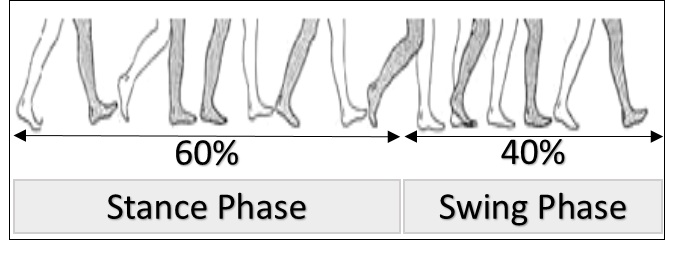
\includegraphics[width=.49\textwidth]{img/gaitlmm2.png}
\caption{Gait Cycle Phases.}
\label{fig:gaitcycles}
\end{figure}

Toledo \textit{et. al}~\cite{toledo2005} compared PD's patients with healthy subjects~\cite{toledo2005,visionbased2009} and identified the PD's patient gait characteristics is having shorter steps, reduction in the joints amplitude and an extension of the stance phase reaching almost $80\%$ for each gait cycle~\cite{ambulatory2010}.

Given that the gait kinetics' studies provide clinical information regarding patient's clinical condition~\cite{gaitusingsensorsreview2012}, we analyzed the signal processing of the sensor raw data of the Parkinson Disease Database~\cite{physionet} to evaluate the PD progress based on the gait characteristics. 

\section{Principal Component Analysis}\label{sec:pca}

Principal Component Analysis (PCA) is a statistic procedure to reduce data and eliminate redundancies. It identifies the data variance and applies linear data transformation to detect the most relevant data components on the first dimension, called the main axis.  The second remaining variance is the secondary axis and so on~\cite{pcarotor2014}.

PCA consists of the following steps~\cite{Shlens05atutorial}: 
\begin{enumerate}
 \item Scale the measurement data into an \textit{m} x \textit{n} matrix, where \textit{m} is the number of measurement types and \textit{n} is the number of samples;
 \item Subtract the mean for each measurement type;
 \item Calculate the \textit{eigenvectors} and \textit{eigenvalues} of the covariance matrix.
 \item The Calculated \textit{eigenvectors} and \textit{eigenvalues} can be used to project the data into a new space called \textit{eigenspace}.
\end{enumerate}


In Figure~\ref{fig:diferencemean}, we show the difference of the mean gait between healthy and PD subjects. We used PCA to identify the difference of the mean gait between PD patients and healthy subjects.

\begin{figure}[!h]
\centering	
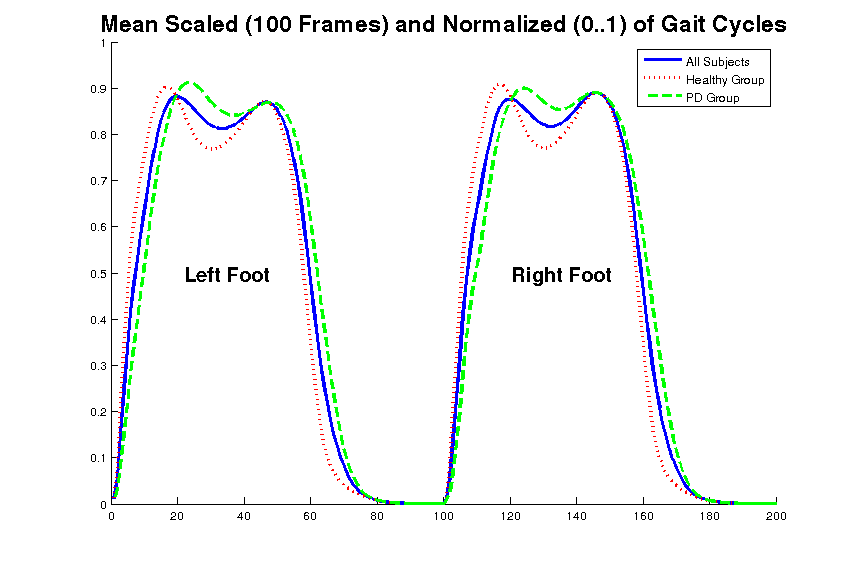
\includegraphics[width=.52\textwidth]{img/meangait.png}
\caption{Mean Vector of the Gait Cycles.}
\label{fig:diferencemean}
\end{figure}




\section{Our Approach}
\label{sec:overview}
The biomechanical analysis of human gait is part of the diagnosis and treatment process for PD. During this analysis, the patients are required to walk. The doctor analyses the gait by looking at the swing and stance phase and the gait posture. To automate the identification of each gait phase in the VGRF data, it is necessary to use signal processing techniques. In this work, we focus on the VGRF of each foot and identifying when the foot initiates contact (i.e., start of stance phase) with the ground and when it is off the ground (i.e., start of swing phase). For this purpose, we used the peaks and valleys technique as shown in details in Section 4.1.

After identifying the cycle, we extract a window length with the cycle movement and the gait characteristics and transform the VGRF data into PCA values. We project the values into the \textit{eigenspace} providing a visualization tool to doctor. With this information, the doctor evaluates the patient's gait.

In Figure~\ref{img:sysarch}, we present an overview of our approach applied to a health monitoring system. Its architecture is composed of the gait system acquisition and signal processing component. The gait acquisition component is responsible for collecting user data and storing them in a database. The signal processing component is responsible for processing the data and making the results available to the healthcare professional.


\begin{figure}[!htb]
	\centering
	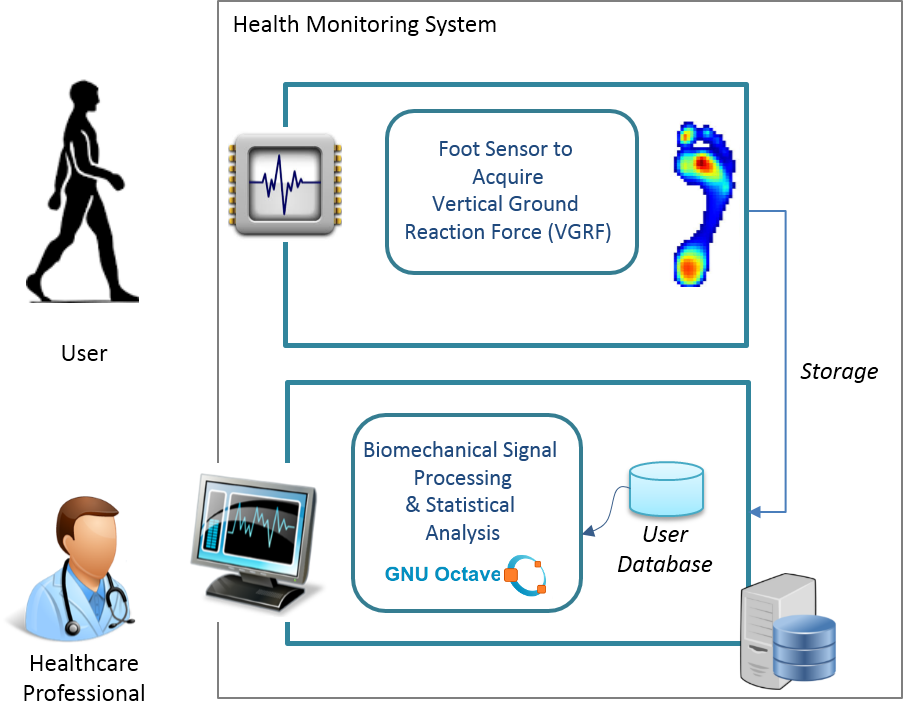
\includegraphics[width=0.475\textwidth]{img/systemoverview.png}
	\caption{System Overview}
	\label{img:sysarch}
\end{figure}

\subsection{Signal Processing Technique}


In this work, we applied peaks and valleys detection technique to identify the beginning and end of each gait cycle. This technique identifies the peaks and discard very low values when they are considered noise. The peak is the highest point between the two lower points, which are considered the cycle valleys. The technique is applied to the signal using low pass filter to remove the signal noise. Thus, our biomechanical signal processing uses raw data, filters noise, identifies motion cycles and extracts feature vector characterizing the motion. Furthermore, we applied machine learning techniques for data classification. The complete process of gait analysis based on PCA is shown in Figure~\ref{fig:biomecproc}. It is divided into two phases: biomechanical signal processing and statistical analysis. 

\begin{figure}[!htb]
	\centering
	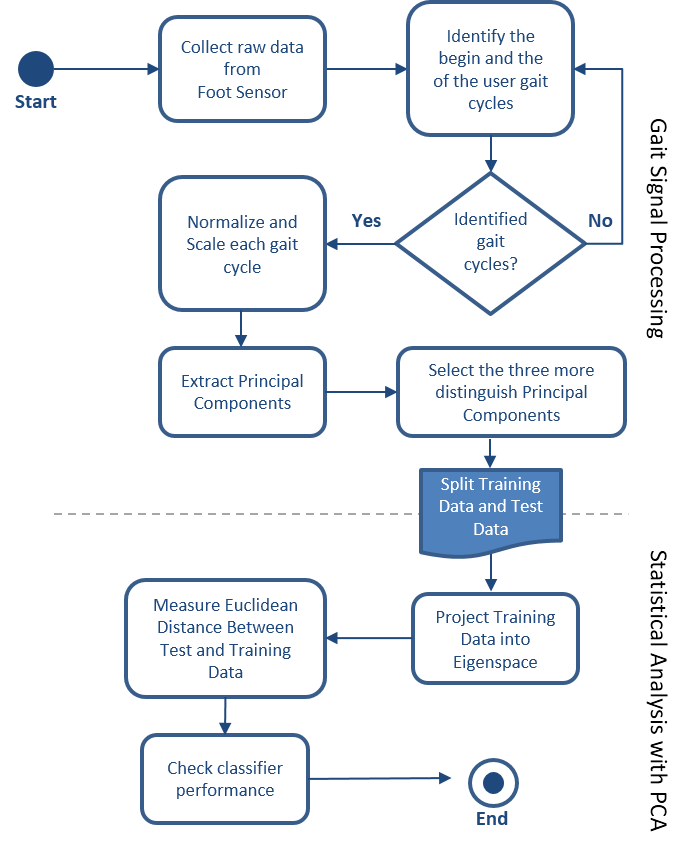
\includegraphics[width=0.475\textwidth]{img/biomecanicalsignal.png}
	\caption{Biomechanical signal processing.}
	\label{fig:biomecproc}
\end{figure}


Considering the periodic movement of the human gait, we applied the peak and valley technique to identify each gait cycle of the raw data as shown in Figure~\ref{fig:peakvalley}. After identifying the gait cycle, we normalized the values from 0 to 1. Calculating the principal components requires a quadratic matrix~\cite{Shlens05atutorial} (\textit{m} x \textit{n}). Therefore, we scaled each gait cycle into 100 frames to generate the principal components and consequently extract the \textit{eigenvalues} and \textit{eigenvectors}. We used a total of 120 gait cycles for each subject.

\begin{figure}[!htb]
	\centering
	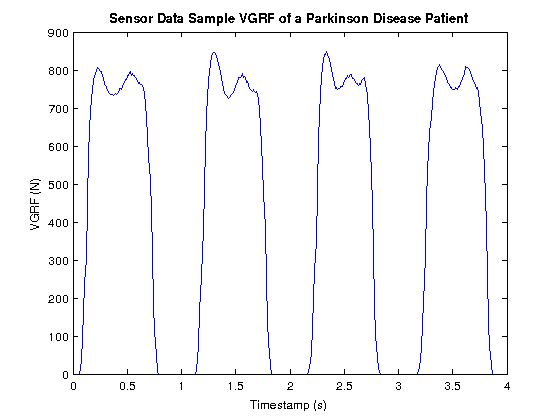
\includegraphics[width=0.475\textwidth]{img/sampleRawData.png}
	\caption{Sample of Acquired Signal of Foot Sensor.}
	\label{fig:peakvalley}
\end{figure}



\section{Material and Methods}\label{sec:mat_methods}
In this work, we used the data available at~{physionet}\footnote{http://physionet.org/pn3/gaitpdb/}, which contains the VGRF records of subjects as they walked at their usual pace for approximately 2 minutes on level ground. To populate this database, data was collected using 8 sensors (Ultraflex Computer Dyno Graphy, Infotronic Inc.\footnote{www.infotronic.nl/items/ExamplesEdwin.pdf}) attached underneath each subject's foot. The sensors measure force (in Newtons) as a function of time. We used two signals, which represent the sum of the 8 sensor outputs for each foot. Even though we used a public database, this work can be adapted to other foot sensors capable of capturing VGRF.

Our source code is under GPL License Version 3.0\footnote{http://www.gnu.org/licenses/gpl-3.0.en.html} and was developed using an Open Source Application (Octave Version 3.8.1\footnote{http://physionet.org/pn3/gaitpdb/}) for numerical computations. The Octave language is similar to Matlab\footnote{http://www.mathworks.com} and most programs are easily portable. To reproduce our results we created a web page containing all the relevant information~\cite{vandewalle2009}\footnote{Website URL: http://gaitparkinson.wordpress.com}. 



We used an open database under the ODC Public Domain Dedication and License (PDDL) v1.0, which allows to freely share, modify, and use this work for any purpose and without any restrictions. We used The Parkinson's Disease database available at~\cite{physionet} to develop a gait analysis system under GPL license to track PD symptoms. Given data quality, we selected data from fifty PD patients and fifty healthy control subjects\footnote{The list of used subjects are described in our Reproducible Research website}. Considering both groups, we had mean age of 66.3 years and 63$\%$ men. We applied signal processing technique for the VGRF signal data acquired by foot sensors. We used a supervised learning approach to train our system to identify the subject group (PD or Control) and with the PCA projection into the \textit{eigenspace} we evaluated the PD's progress through the gait characteristics.

By applying the signal processing techniques, we identified gait cycles and calculated the PCA as our feature vectors. The first three PCA were used in our gait analysis PD's tracking system through the projection of the PCA into the \textit{eigenspace}~\cite{Shlens05atutorial}. Thus, we identified two clusters of the group classes and used the class identification to separate them (i.e. control group and PD patients) as shown in the Figure~\ref{fig:projecaopcaparkinson}. 



\section{Validation}\label{sec:results}

The goal of using PCA for gait analysis is to classify the data and identify the presence of PD. The theory of statistical learning provides a set of techniques for data analysis that allows the acquisition of knowledge by supervised learning methods. PCA~\cite{Shlens05atutorial} is mathematically defined as an orthogonal linear transformation that transforms data into a new coordinate system in which the greatest variance by any projection of data lies along the first coordinate (called the first component), the second greatest variance lies along the second coordinate, and so on. Thus, we used the euclidean distance of the test data to the training data to classify each subject as PD's Group or Control Group. 

In Figure~\ref{fig:projecaopcaparkinson},  we show the projection of the data from both groups, in which the red dots represent PD patients and blue dots, healthy subjects. By analyzing, it is clear that there are two clusters. To verify if the PCA values could be used to track the gait characteristics of a subject, we project the PCA values and draw a trajectory with different measurements of the same person over time, seeing how the symptoms increases or the patient's health improves.

\begin{figure}
  \centering
  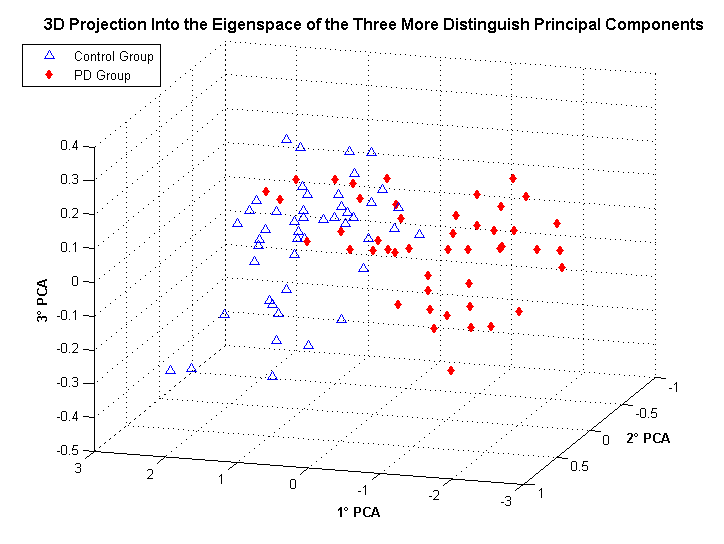
\includegraphics[scale=0.45]{./img/projection-eigenspace.png}
  \caption{Projection of the Three More Distinguish Principal Components}
  \label{fig:projecaopcaparkinson}
\end{figure}

In our analyses the changes in the patient's gait pattern will result in a moving of this point. For instance, if the point moves towards the direction of the subjects with PD's, so the system detects an increase of PD's symptom with the patient.

\begin{figure}
  \centering
  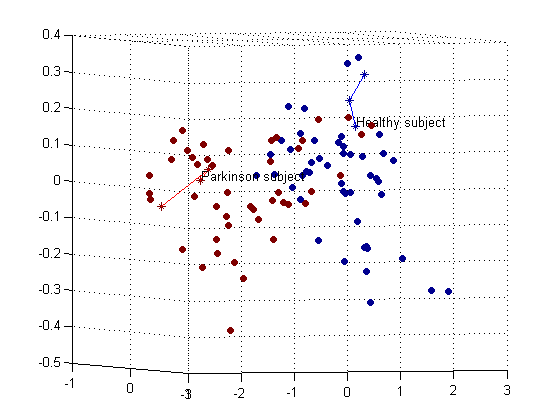
\includegraphics[scale=0.6]{./img/pca-projection-health-parkinson.png}
  \caption{Projection of PD's (RED) and HEALTHY (BLUE dots) Subjects at \textit{eigenspace}. RED and BLUE lines indicate the track of the same subject over time
}
  \label{fig:projecaopcaparkinson}
\end{figure}

For each subject, we defined an ID in the database to design and identify them in the \textit{eigenspace} as shown in Figure~\ref{fig:projecaopcaparkinson}. Using the PCA technique~\cite{Shlens05atutorial}, we identified the two distinct groups of individuals: PD patients and healthy subjects. Changes in one of Parkinson's gait pattern can result in a change of location in the \textit{eigenspace}. If the change is towards data of individuals who do not have the disease, we assume that there was an improvement in the individual state. If it is towards individuals diagnosed with PD, we assume that the model indicates worsening of symptoms.

The calculated distance is the similarity measure and can be expressed by the distance $ D $ \ colon. However, the Euclidean distance, as estimated from the original variables, is influenced by: the scale of measurement, number of variables and the correlation between them. Therefore, standardization of data is necessary to maintain the same variance in the data and be able to identify the similarities~\cite{dillmann2014}. In this research, the results were evaluated by means of the Euclidean distance between the vector of a test subject designed in the \textit{eigenspace}, compared to all individuals in the training group. So, if the test subject is closer to an individual diagnosed with PD, he/she is classified as PD's subject. On the other hand, if the test subject is closer to an individual without the diagnosis of PD, he/she is classified as a control subject.




\subsection{Cross-Validation Results}
To verify the accuracy of the classification of healthy versus PD, we performed Cross-validation~\cite{datamining2005}. Cross-validation is a technique used to assess the generalization of a prediction model in a data set. At first, it holds the partition data set into mutually exclusive subsets and then this subset is used to verify the accuracy of the search model.


To prevent over-fitting, accuracy is measured using a leave-one-out cross-validation. We hold a subject as the test data and the remainder group we used as training. The choice of the training group includes all classes in the database~\cite{datamining2005}. This technique is widely used to mitigate the occurrence of bias in research, because the training process is repeated several times with different samples including different cases in each class. Given a single sample, a method of prediction error rate in machine learning is to use a leave-one-out cross-validation~\cite{datamining2005}.

To test the accuracy of the PCA method with cross-validation, we applied it to classify the data in the database, resulting in 81.00$\%$ of accuracy.

The classification performance obtained in this study is presented in the confusion matrix for two classes which consists of a matrix $2$\ x $2$\, with (TP, FP, TN and FN) presented in Table~\ref{table:resultadomatrizconfusaosvm}. A true positive (TP) indicates correctly classified with abnormal movement, true negative (TN) indicates correctly classified with normal movement. 

Accordingly, the false positives (FP) indicate the normal movement classified as abnormal ones and the false negatives (FN) indicate the real abnormal movement not correctly detected. Table~\ref{table:metricas} shows the classification performance, where the \textit{TpRate} is TP divided by the total number of positives, which is TP + FN; the \textit{FpRate} is FP divided by the total number of negatives, which is FP + TN. The \textit{Accuracy} is the number of correct classifications divided by the total number of samples~\cite{datamining2005}.

\begin{table}[!htbp]
\caption{Confusion Matrix Of PCA Classification Leave-One-Out Cross Validation}
\label{table:resultadomatrizconfusaosvm}
\centering
\begin{tabular}{l|c|c|}
\cline{2-3}
\multicolumn{1}{c}{}                         & \multicolumn{2}{|c|}{\textit{\textbf{Predicted Class}}} \\ \cline{2-3} 
                                             & \textbf{Parkinson}      & \textbf{Control Group}         \\ \hline
\multicolumn{1}{|l|}{\textbf{Parkinson}} & 43       & 7          \\ \hline
\multicolumn{1}{|l|}{\textbf{Control Group}}     & 12           & 38     \\ \hline
\end{tabular}
\end{table}


\begin{table}[htbp!]
\caption{Performance of PD's and Control Group classification}
\label{table:metricas}
\centering
\begin{tabular}{|l|r|}
\hline
\multicolumn{2}{|l|}{\textbf{Classifier Metrics}} \\ \hline
\textbf{TpRate}                    & 86.00$\%$\                 \\ \hline
\textbf{FpRate}                    & 24.00$\%$\                \\ \hline
\textbf{Precision}                 & 78.18$\%$\                \\ \hline
\textbf{Accuracy}                  & 81.00$\%$\                \\ \hline
\textbf{F-Score}                 & 81.90$\%$\                \\ \hline
\end{tabular}
\end{table}


\section{Conclusion}\label{sec:conclusion}

In this work, a gait analysis approach to track Parkinson's Disease evolution by monitoring walking abnormalities. This approach was evaluated by assessing the biomechanical data measurements from a public database~\cite{physionet}. We monitored PD gait symptoms extracting each gait cycle and calculating their respective Principal Components.  

To evaluate our approach, we performed an experimental study with 100 research subjects divided into PD and Control groups. We used PCA and the euclidean distance to identify PD's gait characteristics and had an accuracy of 81.00\% and 86.00\% of \textit{TpRate}. 

Our study's limitation is that we do not consider the variation of gait movement between different people. Therefore, it is not a conclusive test to diagnose PD~\cite{gaitusingsensorsreview2012, national2006parkinson}. Despite this limitation, it is accurate to track PD's symptoms based on the user gait.

For future works, we plan to use another public database hosted on Physionet~\cite{physionet} including different diseases as: Huntington's Disease, Amyotrophic Lateral Sclerosis and Stroke patients\footnote{http://www.physionet.org/physiobank/database/gaitndd/} to perform multi-class classification. 



\bibliographystyle{IEEEtran}
\bibliography{sigproc,IEEEFormat}


% that's all folks
\end{document}


